% SciPy 数值微分与积分
\pentry{Python 入门\upref{Python}}
\verb|SciPy|函数库在\verb|NumPy|库\upref{numpy}的基础上增加了众多的数学、科学以及工程计算中常用的库函数.例如线性代数\upref{Vector}、常微分方程数值求解\upref{OdeNum}、信号处理、图像处理、稀疏矩阵\upref{SprMat}等等.
使用\verb|SciPy|库之前需要先导入库,
\begin{lstlisting}[language=python]
import  scipy#导入scipy中所有模块
from scipy import integrate#导入其中积分模块
\end{lstlisting}
\subsection{数值积分}
数值积分是对定积分的数值求解.例如可以利用数值积分计算某个形状的面积.下面让我们来考虑一下如何计算半径为1的半圆的面积,根据圆的面积公式,其面积应该等于$\pi$.单位半圆曲线可以用函数\verb|half_circle()|表示, 对应计算积分的代码如下:
\begin{lstlisting}[language=python]
def half_circle(x):
    return (1-x**2)**0.5

from scipy import integrate
res, err = integrate.quad(half_circle, -1, 1)
print(res,err)
输出:
1.5707963267948983 1.0002354500215915e-09
\end{lstlisting}
此处调用了积分模块下的\verb|quad|函数, 这里不仅返回了积分结果,还给出来计算误差.多重定积分的求值可以通过多次调用\verb|quad|函数实现, 为了调用方便, \verb|integrate|库提供了\verb|dblquad|函数
进行二重定积分, \verb|tplquad|函数进行三重定积分.

\verb|dblquad|函数的调用方式为:
\begin{lstlisting}[language=python]
dblquad(func2d, a, b, gfun, hfun)
\end{lstlisting}
对于\verb|func2d(x,y)|函数进行二重积分, 其中\verb|a,b|为变量$x$的积分区间,而\verb|gfun(x)|到\verb|hfun(x)|为变量$y$的积分区间.

\verb|tblquad|函数的调用方式与上面一样.

\subsection{数值解微分方程组}
\verb|scipy.integrate|库提供了数值积分和常微分方程组求解算法\verb|odeint|.
\verb|odeint()|函数需要至少三个变量, 第一个是微分方程函数, 第二个是微分方程初值, 第三个是微分的自变量.

下面让我们来看看如何用\verb|odeint|计算十分经典的洛仑兹吸引子的轨迹. 洛仑兹吸引子由下面的三个微分方程定义:
\begin{align}
&\dot{x}=\sigma\\
&\dot{y}=x(\rho-y\\
&\dot{z}=xy-\beta
\end{align}
\begin{lstlisting}[language=python]
from scipy.integrate import odeint
import numpy as np
def lorenz(w, t, p, r, b):
    # 给出位置矢量w,和三个参数p, r, b计算出
    # dx/dt, dy/dt, dz/dt的值
    x, y, z = w
    # 直接与lorenz的计算公式对应
    return np.array([p*(y-x), x*(r-z)-y, x*y-b*z])

t = np.arange(0, 30, 0.01) # 创建时间点
# 调用ode对lorenz进行求解, 用两个不同的初始值
track1 = odeint(lorenz, (0.0, 1.00, 0.0), t, args=(10.0, 28.0, 3.0))
track2 = odeint(lorenz, (0.0, 1.01, 0.0), t, args=(10.0, 28.0, 3.0))
from mpl_toolkits.mplot3d import Axes3D
import matplotlib.pyplot as plt
fig = plt.figure()
ax = Axes3D(fig)
ax.plot(track1[:,0], track1[:,1], track1[:,2])
ax.plot(track2[:,0], track2[:,1], track2[:,2])
plt.show()
\end{lstlisting}
结果如\autoref{SciPy_fig1}所示.
\begin{figure}[ht]
\centering
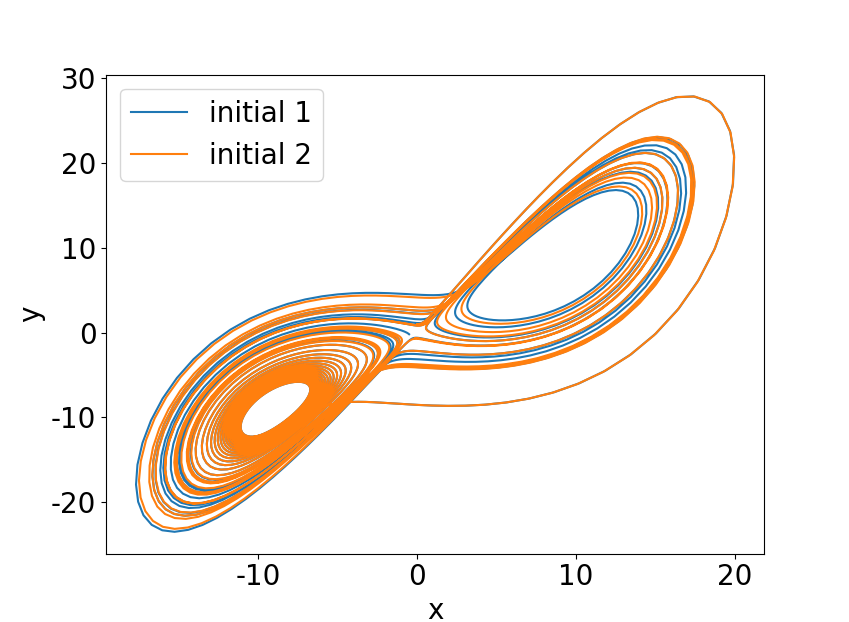
\includegraphics[width=8cm]{./figures/SciPy_1.png}
\caption{洛伦兹微分方程数值解} \label{SciPy_fig1}
\end{figure}
这里我们还使用到了第四个参数\verb|args|, 它是一个\verb|tuple|类型,给函数传递额外的参数. 我们看到即使初始值只相差0.01,两条运动轨迹也是完全不同的.
在程序中先定义一个\verb|lorenz|函数,它的任务是计算出某个位置的各个方向的微分值,这个计算直接根据洛仑兹吸引子的公式得出.然后调用\verb|odeint|,对微分方程求解,\verb|odeint|有许多参数,这里用到的四个参数分别为:\\
1. \verb|lorenz|, 它是计算某个位移上的各个方向的速度(位移的微分);\\
2. \verb|(0.0, 1.0, 0.0)|, 位移初始值.计算常微分方程所需的各个变量的初始值;\\
3. \verb|t|, 表示时间的数组,\verb|odeint|对于此数组中的每个时间点进行求解,得出所有时间点的位置;\\
4. \verb|args|, 这些参数直接传递给\verb|lorenz|函数,因此它们都是常量.